% !TEX encoding = UTF-8
% !TEX TS-program = pdflatex
% !TEX root = ../tesi.tex

%**************************************************************
\chapter{Analisi dei requisiti}
\label{cap:analisi-requisiti}
%**************************************************************

\intro{In questo capitolo vengono definite con precisione le funzionalità del software che è stato prodotto durante lo stage. Viene presentata l'analisi dei requisiti svolta per il progetto, approfondita con i diagrammi dei casi d'uso.}\\

\section{Casi d'uso}
I diagrammi dei casi d'uso (in inglese, \textit{Use Case Diagram}) sono diagrammi di tipo \gls{umlg} che servono a descrivere le interazioni fra il sistema software e gli utenti che lo utilizzano, mostrando l'insieme funzionalità esposte dal sistema dal punto di vista degli utenti. \\
Poiché lo stage era incentrato sull'estensione del framework e lo sviluppo di un algoritmo euristico per la risoluzione dei problemi di scheduling, la prima parte del progetto non necessitava di esporre funzionalità all'utente. D'altro canto, una volta sviluppata l'applicazione per risolvere il problema specifico del casinò, avrei dovuto garantire dei servizi minimi all'utente per inserire l'input (informazioni circa le postazioni, i lavoratori, i turni, etc...) e mostrare l'output (lo scheduling prodotto). \\
Per questo motivo i diagrammi dei casi d'uso risultano minimali e in numero ridotto.\\
\\
Ogni caso d'uso è classificato secondo la seguente convenzione:
\begin{center}
    UC[Codice padre]*.[Codice identificativo]
\end{center}

\begin{itemize}
    \item \textbf{Codice padre}: \MakeUppercase{} il codice identificativo del caso d'uso generico che ha generato il caso d'uso in esame. Se il caso d'uso non è stato generato da altri, va tralasciato;
    \item \textbf{Codice identificativo}: Identifica univocamente il caso d'uso. \MakeUppercase{è} un codice composto da sole cifre. 
\end{itemize}
\noindent
Alcuni casi d'uso possono essere associati ad un diagramma dei casi d'uso riportante lo stesso titolo e codice.
\clearpage
\subsection{Diagrammi dei casi d'uso}
\begin{figure}[!h]
    \begin{widepage}
        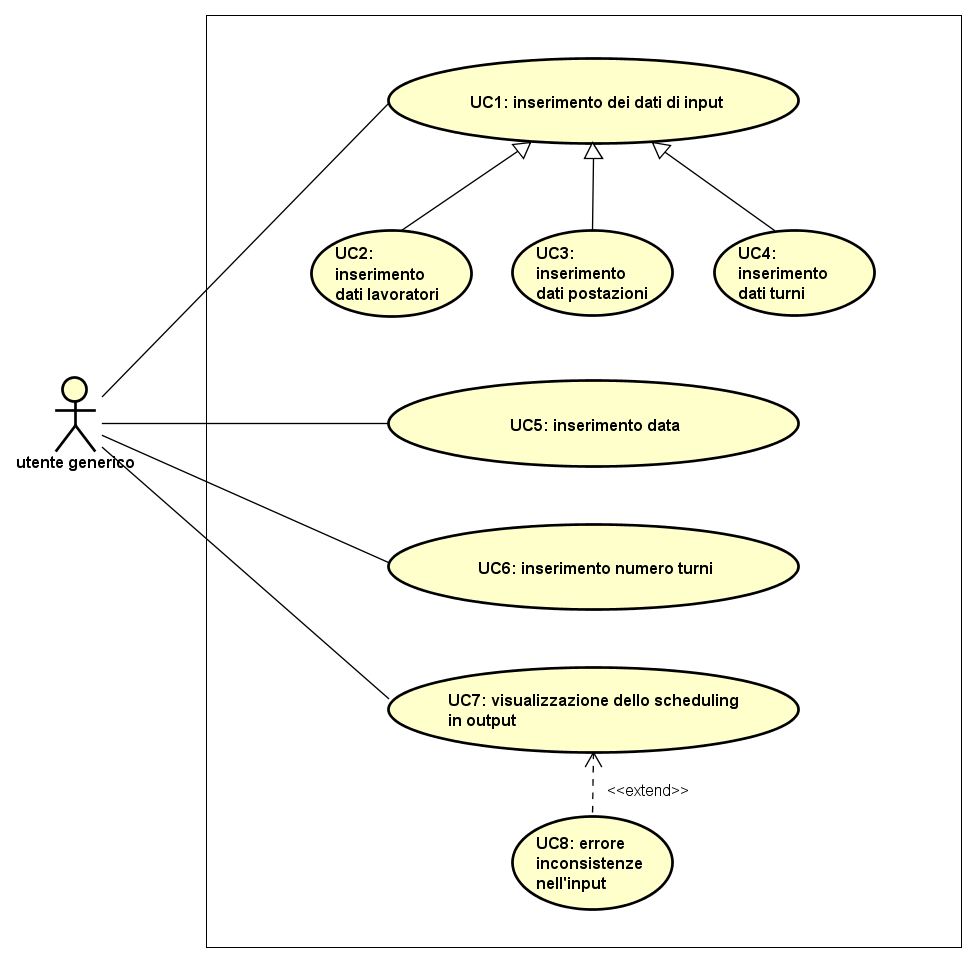
\includegraphics[width=17cm,keepaspectratio]{../immagini/usecase/System.png}
        \caption{Diagramma dei casi d'uso ad alto livello}
    \end{widepage}
\end{figure}
\clearpage
\subsection{UC1: Inserimento dei dati di input}
\label{UC1}
\begin{itemize}
    \item \textbf{Attori}: utente generico;
    \item \textbf{Descrizione}: l'utente inserisce i dati in input al programma per realizzare uno scheduling.
    \item \textbf{Generalizzazioni}: l'utente inserisce i dati in input al programma per realizzare uno scheduling riguardati i lavoratori (UC2), le postazioni (UC3), i turni (UC4).
\end{itemize}

\subsection{UC2: Inserimento dati lavoratori}
\label{UC2}
\begin{figure}[!h]
    \begin{widepage}
    \def\svgwidth{\columnwidth}
    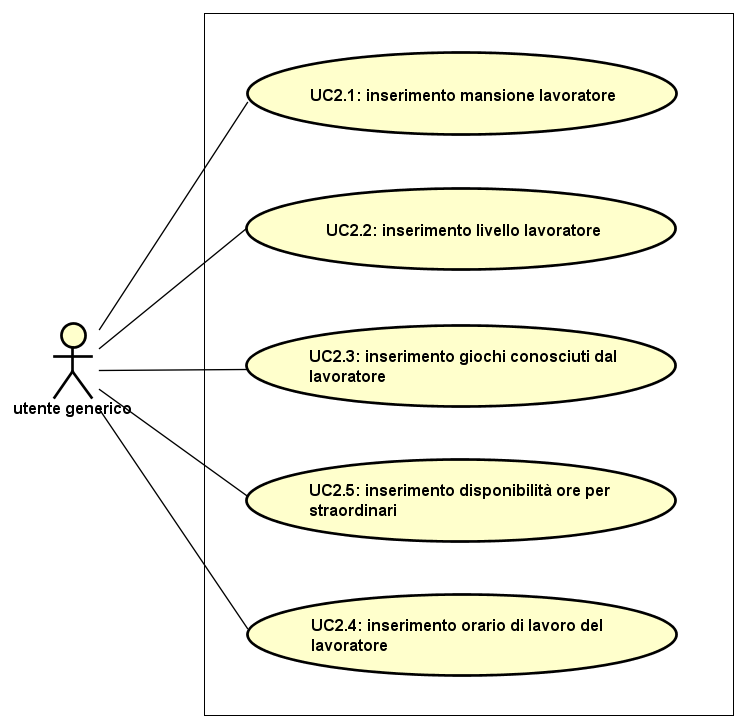
\includegraphics[width=14.9cm,keepaspectratio]{../immagini/usecase/UC2.png}
    \caption{UC2: Inserimento dati lavoratori}
    \end{widepage}
\end{figure}
\clearpage
\begin{itemize}
    \item \textbf{Attori}: utente generico;
    \item \textbf{Descrizione}: l'utente inserisce i dati in input al programma per realizzare uno scheduling riguardanti i lavoratori.
\end{itemize}
\paragraph{UC2.1: Inserimento mansione lavoratore}
\begin{itemize}
    \item \textbf{Attori}: utente generico;
    \item \textbf{Descrizione}: l'utente inserisce i dati in input al programma circa la mansione del lavoratore (dealer, dealer-inspector, inspector).
\end{itemize}
\paragraph{UC2.2: Inserimento livello lavoratore}
\begin{itemize}
    \item \textbf{Attori}: utente generico;
    \item \textbf{Descrizione}: l'utente inserisce i dati in input al programma circa il livello del lavoratore (dealer: 1-8, dealer-inspector: 3, inspector: 1-3).
\end{itemize}
\paragraph{UC2.3: Inserimento giochi conosciuti dal lavoratore}
\begin{itemize}
    \item \textbf{Attori}: utente generico;
    \item \textbf{Descrizione}: l'utente inserisce i dati in input al programma circa i giochi conosciuti dal lavoratore.
\end{itemize}
\paragraph{UC2.4: Inserimento orario di lavoro del lavoratore}
\begin{itemize}
    \item \textbf{Attori}: utente generico;
    \item \textbf{Descrizione}: l'utente inserisce i dati in input al programma circa l'orario di lavoro del giocatore (ora di inizio, ora di fine).
\end{itemize}
\paragraph{UC2.5: Inserimento disponibilità ore per straordinari}
\begin{itemize}
    \item \textbf{Attori}: utente generico;
    \item \textbf{Descrizione}: l'utente inserisce i dati in input al programma circa la disponibilità a svolgere straordinari (ore).
\end{itemize}
\clearpage
\subsection{UC3: Inserimento dati postazioni}
\label{UC3}
\begin{figure}[!h]
    \def\svgwidth{\columnwidth}
    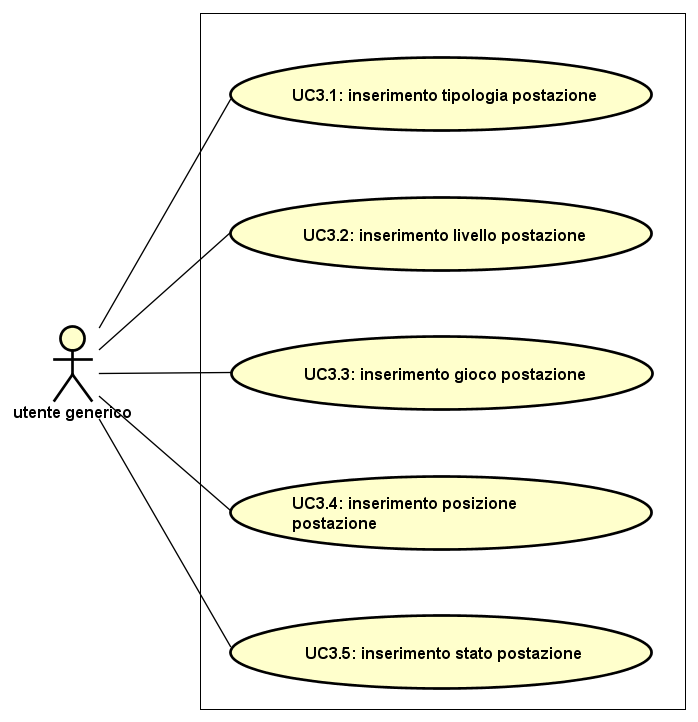
\includegraphics[width=\textwidth]{../immagini/usecase/UC3.png}
    \caption{UC3: Inserimento dati postazioni}
\end{figure}
\FloatBarrier
\noindent
\begin{itemize}
    \item \textbf{Attori}: utente generico;
    \item \textbf{Descrizione}: l'utente inserisce i dati in input al programma per realizzare uno scheduling riguardanti le postazioni.
\end{itemize}
\paragraph{UC3.1: Inserimento tipologia postazione}
\begin{itemize}
    \item \textbf{Attori}: utente generico;
    \item \textbf{Descrizione}: l'utente inserisce i dati in input al programma circa la tipologia della postazione (tavolo, pit).
\end{itemize}
\paragraph{UC3.2: Inserimento livello postazione}
\begin{itemize}
    \item \textbf{Attori}: utente generico;
    \item \textbf{Descrizione}: l'utente inserisce i dati in input al programma circa il livello della postazione (tavoli: 1-8, pit: 1-3).
\end{itemize}
\paragraph{UC3.3: Inserimento gioco postazione}
\begin{itemize}
    \item \textbf{Attori}: utente generico;
    \item \textbf{Descrizione}: l'utente inserisce i dati in input al programma circa il gioco che si gioca nella postazione.
\end{itemize}
\paragraph{UC3.4: Inserimento posizione postazione}
\begin{itemize}
    \item \textbf{Attori}: utente generico;
    \item \textbf{Descrizione}: l'utente inserisce i dati in input al programma circa la posizione che si assume lavorando nella postazione (seduta, in piedi).
\end{itemize}
\paragraph{UC3.5: Inserimento stato}
\begin{itemize}
    \item \textbf{Attori}: utente generico;
    \item \textbf{Descrizione}: l'utente inserisce i dati in input al programma circa lo stato della postazione (aperta, chiusa).
\end{itemize}
\subsection{UC4: Inserimento dati turni}
\label{UC4}
\begin{figure}[!h]
    \def\svgwidth{\columnwidth}
    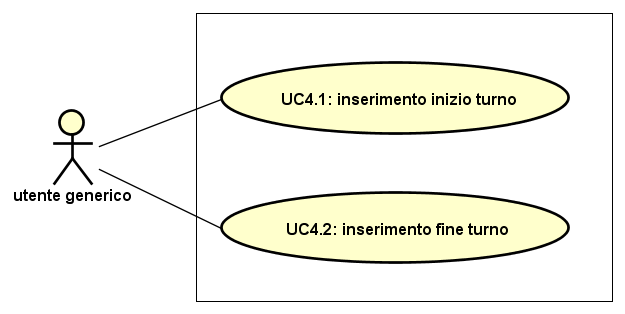
\includegraphics[width=\textwidth]{../immagini/usecase/UC4.png}
    \caption{UC4: Inserimento dati turni}
\end{figure}
\FloatBarrier
\noindent
\begin{itemize}
    \item \textbf{Attori}: utente generico;
    \item \textbf{Descrizione}: l'utente inserisce i dati in input al programma per realizzare uno scheduling riguardanti i turni.
\end{itemize}
\paragraph{UC4.1: Inserimento inizio turno}
\begin{itemize}
\item \textbf{Attori}: utente generico;
\item \textbf{Descrizione}: l'utente inserisce i dati in input al programma circa l'ora di inizio di un turno.
\end{itemize}
\paragraph{UC4.2: Inserimento fine turno}
\begin{itemize}
\item \textbf{Attori}: utente generico;
\item \textbf{Descrizione}: l'utente inserisce i dati in input al programma circa l'ora di fine di un turno.
\end{itemize}

\subsection{UC5: Inserimento data}
\label{UC5}
\begin{itemize}
    \item \textbf{Attori}: utente generico;
    \item \textbf{Descrizione}: l'utente inserisce la data per la quale vuole trovare uno scheduling (importante perché gli orari del personale possono variare di data in data).
    \item \textbf{Scenario alternativo}: se l'utente non inserisce una data, viene trovato lo scheduling per il giorno corrente.
\end{itemize}

\subsection{UC6: Inserimento numero turni}
\label{UC6}
\begin{itemize}
    \item \textbf{Attori}: utente generico;
    \item \textbf{Descrizione}: l'utente inserisce il numero di turni per il quale vuole trovare uno scheduling.
    \item \textbf{Scenario alternativo}: se l'utente non inserisce un numero, viene trovato lo scheduling per tutti i turni.
\end{itemize}

\subsection{UC7: Visualizzazione dello scheduling in output}
\label{UC7}
\begin{itemize}
    \item \textbf{Attori}: utente generico;
    \item \textbf{Descrizione}: l'utente visualizza l'output del programma (soluzione ammissibile o non).
    \item \textbf{Estensioni}: non c'è output perché è stato commesso un errore di inserimento dei dati.
\end{itemize}
\clearpage
%***********************************************************************
\section{Tracciamento dei requisiti}

Da un'attenta analisi dei requisiti e degli use case effettuata sul progetto è stata stilata la tabella che traccia i requisiti in rapporto agli use case.\\
Sono stati individuati diversi tipi di requisiti e si è quindi fatto utilizzo di un codice identificativo per distinguerli.\\
Il codice dei requisiti è così strutturato R(F/Q/V)(N/D/O) dove:
\begin{enumerate}
	\item[R =] requisito
    \item[F =] funzionale
    \item[Q =] qualitativo
    \item[V =] di vincolo
    \item[N =] obbligatorio (necessario)
    \item[D =] desiderabile
    \item[Z =] opzionale
\end{enumerate}
Nelle tabelle \ref{tab:requisiti-funzionali}, \ref{tab:requisiti-qualitativi} e \ref{tab:requisiti-vincolo} sono riassunti i requisiti e il loro tracciamento con gli use case delineati in fase di analisi.

\newpage

\begin{table}%
\caption{Tabella del tracciamento dei requisti funzionali}
\label{tab:requisiti-funzionali}
\begin{tabularx}{\textwidth}{lXl}
\hline\hline
\textbf{Requisito} & \textbf{Descrizione} & \textbf{Use Case}\\
\hline
RFN-1     & L'interfaccia permette di configurare il tipo di sonde del test & UC1 \\
\hline
\end{tabularx}
\end{table}%

\begin{table}%
\caption{Tabella del tracciamento dei requisiti qualitativi}
\label{tab:requisiti-qualitativi}
\begin{tabularx}{\textwidth}{lXl}
\hline\hline
\textbf{Requisito} & \textbf{Descrizione} & \textbf{Use Case}\\
\hline
RQD-1    & Le prestazioni del simulatore hardware deve garantire la giusta esecuzione dei test e non la generazione di falsi negativi & - \\
\hline
\end{tabularx}
\end{table}%

\begin{table}%
\caption{Tabella del tracciamento dei requisiti di vincolo}
\label{tab:requisiti-vincolo}
\begin{tabularx}{\textwidth}{lXl}
\hline\hline
\textbf{Requisito} & \textbf{Descrizione} & \textbf{Use Case}\\
\hline
RVO-1    & La libreria per l'esecuzione dei test automatici deve essere riutilizzabile & - \\
\hline
\end{tabularx}
\end{table}%